\documentclass{article}

\usepackage{graphicx}
\usepackage{tikz}
\usepackage{tikzsymbols}
\usetikzlibrary{calc,patterns,shapes.geometric}
\pagestyle{empty}
\usepackage[margin=0pt]{geometry}
\geometry{papersize={14in,12in}}

\def\centerarc[#1](#2)(#3:#4:#5){\draw[#1] ($(#2)+({#5*cos(#3)},{#5*sin(#3)})$) arc (#3:#4:#5);}

\begin{document}
	\begin{figure}
		\centering
		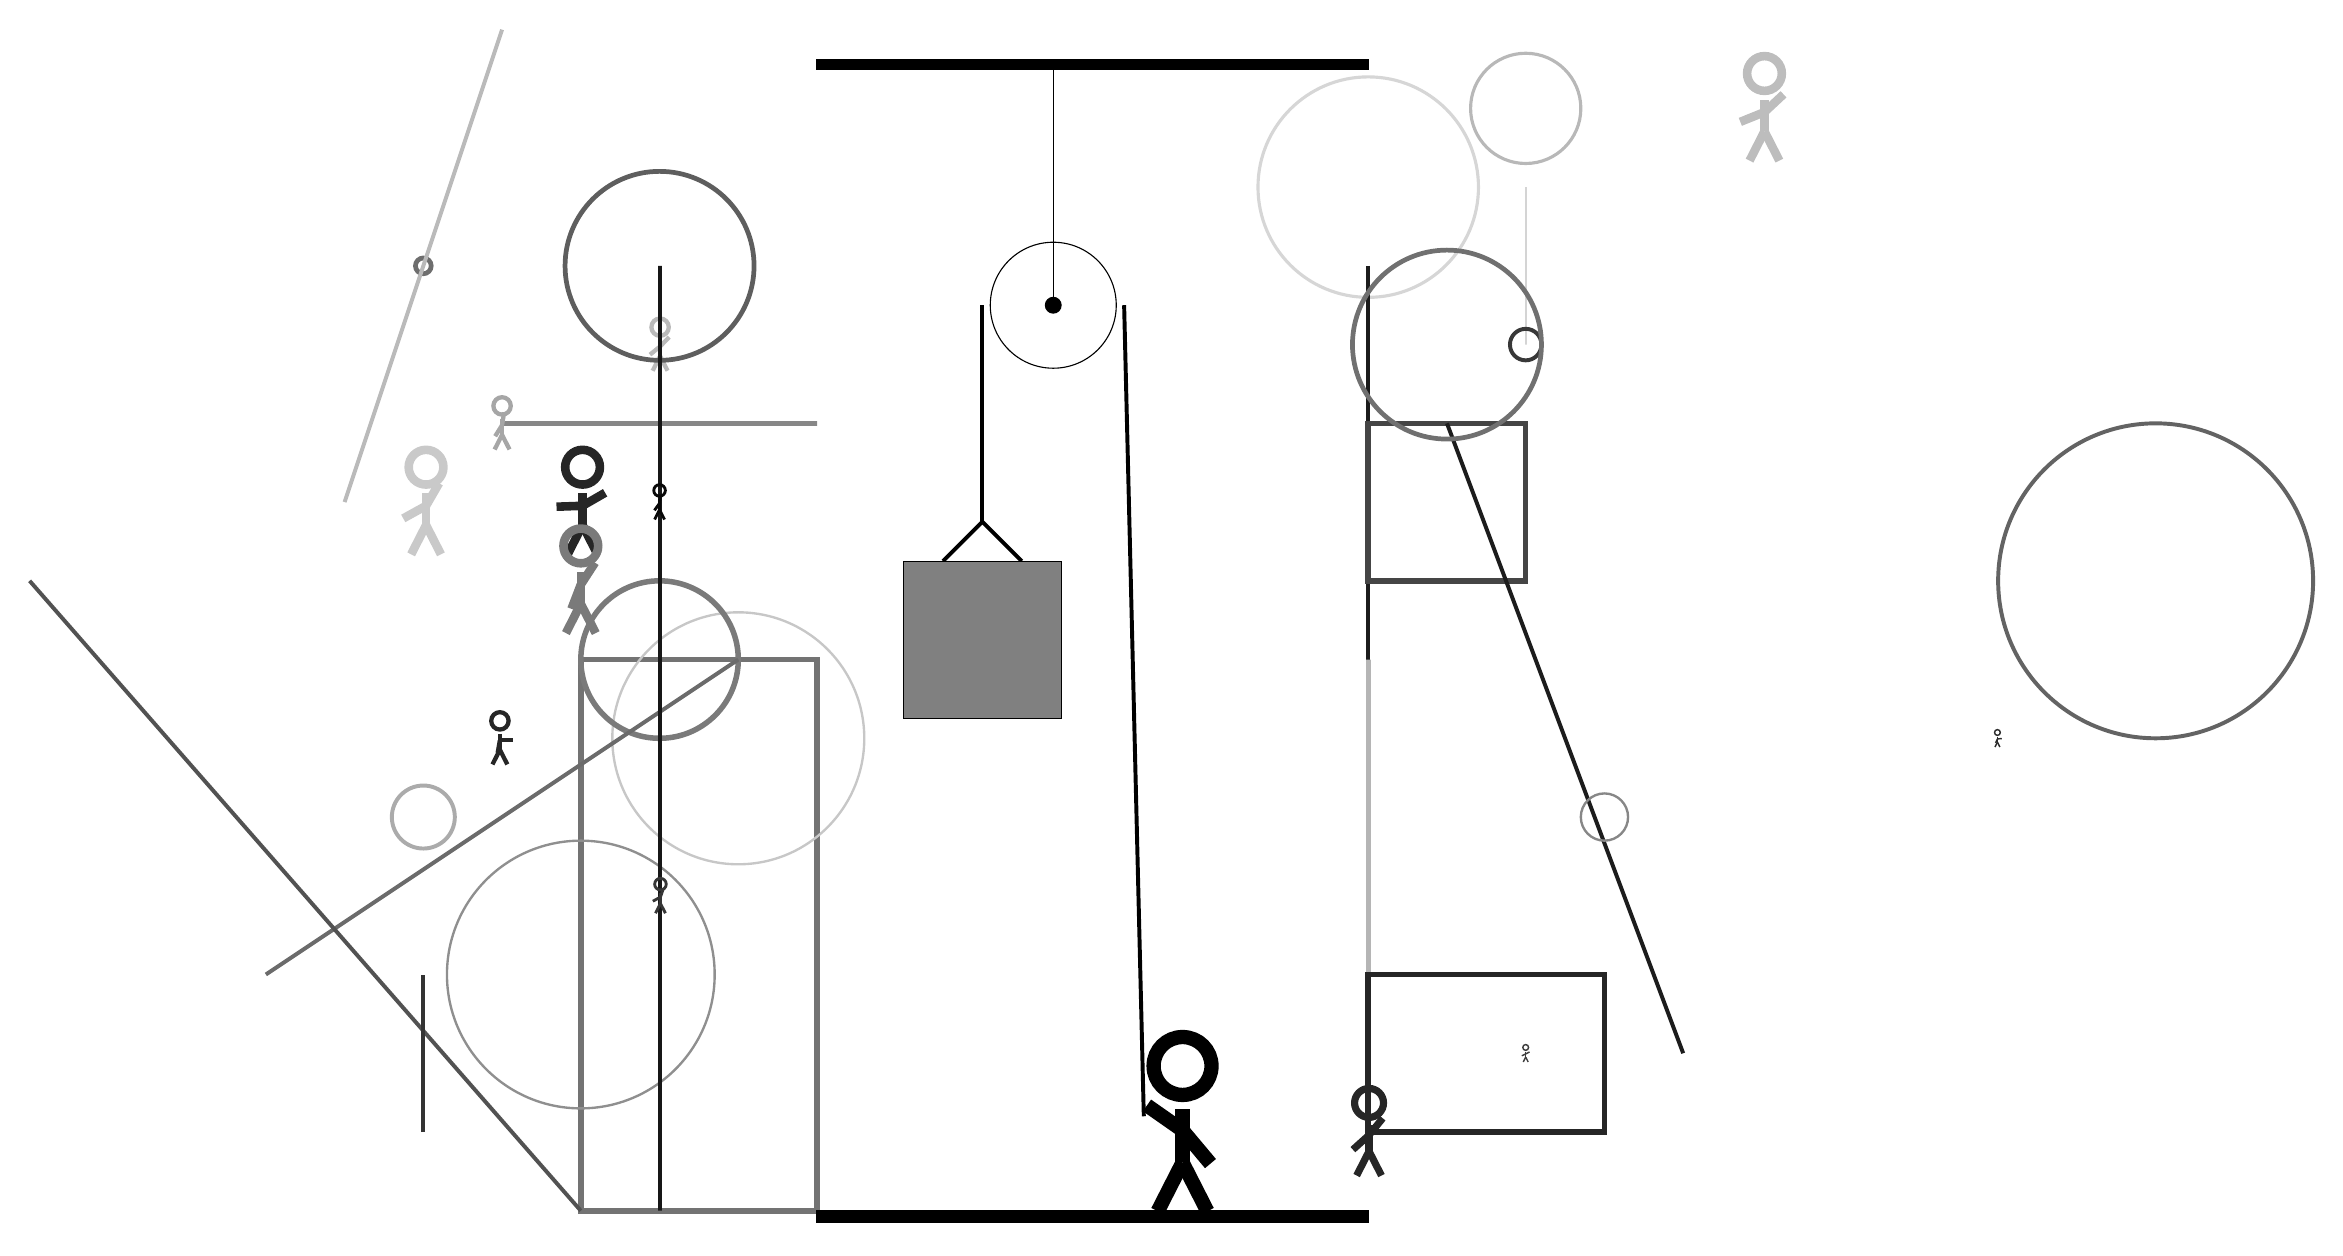
\begin{tikzpicture}
			%%%%% START %%%%%
			
			\draw[fill=black] (-2, 11.5) rectangle (5, 11.625);
			
			\node[line width=0.4mm, color=black!27] at (-4, 8) {\Strichmaxerl[3][39][46]};
			
			\node[line width=0.2mm, color=black!85] at (-6, 3) {\Strichmaxerl[3][80][0]};
			\node[line width=0.3mm, color=black!83] at (13, 3) {\Strichmaxerl[1][65][5]};
			\draw[line width=0.7mm, color=black!55] (-2, 4) rectangle (-5, -3);
			\node[line width=0.4mm, color=black!76] at (7, -1) {\Strichmaxerl[1][26][26]};
			\draw [line width=0.3mm, color=black!22](-3, 3) circle (1.6);
			
			\node[line width=0.3mm, color=black!85] at (5, -2) {\Strichmaxerl[5][42][51]};
			
			\draw [line width=0.6mm, color=black!57](-7, 9) circle (0.1);
			\draw [line width=0.7mm, color=black!52](-4, 4) circle (1.0);
			\draw[line width=0.2mm, color=black!17] (7, 8) rectangle (7, 10);
			\draw [line width=0.5mm, color=black!61](15, 5) circle (2.0);
			\draw [line width=0.3mm, color=black!44](-5, 0) circle (1.7);
			\draw[line width=0.7mm, color=black!47] (-2, 7) rectangle (-6, 7);
			
			\node[line width=0.7mm, color=black!85] at (-5, 6) {\Strichmaxerl[6][2][30]};
			\draw [line width=0.4mm, color=black!16](5, 10) circle (1.4);
			\node[line width=0.7mm, color=black!35] at (-6, 7) {\Strichmaxerl[3][58][81]};
			
			\draw[line width=0.5mm, color=black!58](-3, 4) -- (-9, 0);
			\node[line width=0.3mm, color=black!26] at (10, 11) {\Strichmaxerl[6][22][43]};
			\draw [line width=0.5mm, color=black!78](7, 8) circle (0.2);
			
			\draw[line width=0.5mm, color=black!89](5, 9) -- (5, -2);
			\draw[line width=0.7mm, color=black!73] (5, 7) rectangle (7, 5);
			\draw[line width=0.5mm, color=black!27](-6, 12) -- (-8, 6);
			\node[line width=0.3mm, color=black!21] at (-7, 6) {\Strichmaxerl[6][29][60]};
			\draw[line width=0.5mm, color=black!68](-5, -3) -- (-12, 5);
			\draw[line width=0.5mm, color=black!89](9, -1) -- (6, 7);
			\draw[line width=0.6mm, color=black!29] (5, -2) rectangle (5, 4);
			\draw [line width=0.6mm, color=black!56](6, 8) circle (1.2);
			\draw [line width=0.5mm, color=black!33](-7, 2) circle (0.4);
			
			\draw[line width=0.5mm, color=black!80](-7, -2) -- (-7, 0);
			
			\draw [line width=0.6mm, color=black!63](-4, 9) circle (1.2);
			\draw[line width=0.5mm, color=black!91] (-4, -3) rectangle (-4, 9);
			
			\draw[line width=0.7mm, color=black!85] (5, -2) rectangle (8, 0);
			\node[line width=0.3mm, color=black!97] at (-4, 6) {\Strichmaxerl[2][54][84]};
			\node[line width=0.6mm, color=black!52] at (-5, 5) {\Strichmaxerl[6][69][57]};
			\draw [line width=0.3mm, color=black!47](8, 2) circle (0.3);
			\draw [line width=0.4mm, color=black!28](7, 11) circle (0.7);
			
			\node[line width=0.5mm, color=black!79] at (-4, 1) {\Strichmaxerl[2][29][71]};
			
			\draw (1, 8.5) circle (0.8);
			\draw[fill=black] (1, 8.5) circle (0.1);
			\draw (1, 11.5) -- (1, 8.5);
			
			\draw[line width=0.5mm] (-0.4, 5.25) -- (0.1, 5.75) -- (0.6, 5.25);
			\draw[fill=black!50] (-0.9, 5.25) rectangle (1.1, 3.25);
			
			\draw[line width=0.5mm] (0.1, 8.5) -- (0.1, 5.75);
			\centerarc[line width=0.5mm](1, 8.5)(0:180:0.9);
			\draw[line width=0.5mm](1.9, 8.5) -- (2.15, -1.8);
			
			\node at (2.6, -1.9) {\Strichmaxerl[10][-35][-50]};
			
			\draw[fill=black] (-2, -3) rectangle (5, -3.15);
			
			%%%%% END %%%%%
		\end{tikzpicture}
	\end{figure}	
\end{document}